Hiring effectively is one of the key challenges faced by any organization.
There are two possibly conflicting optimization issues that a hiring committee faces when considering a candidate: 
(i) the value added to the organization in terms of the candidate's raw skills and competencies, and 
(ii) how well the candidate can collaborate with the existing members of the organization.
The first consideration depends on the complementarity between the candidate's skills and the tasks that the organization aims to complete. 
This is called \textit{utility} in the team formation literature.
The second consideration is commonly known as the \textit{communication cost}.

In their seminal paper, Lappas et al. \cite{lappas2009finding} first introduced the problem of \textit{team formation}, where they modeled team in the form of a graph.
They proposed two graph distance-based measures of communication cost, namely the diameter and minimum spanning tree of the graph. 
They showed that the team formation problem is NP-Hard for both types of communication costs. 
Subsequent works  \cite{sozio2010community, kargar2011discovering, anagnostopoulos2010power, rangapuram2013towards} explored more realistic formulations of the team formation problem. They study different cost functions and objectives that model the real world requirements more closely.
In \cite{bhowmik2014submodularity}, a submodular variant of the team formation problem is proposed, enabling an approximation guarantee for a simulated annealing algorithm.

Our work distinguishes itself by studying the problem of team formation from an organization's point of view. The major challenges that an organizational perspective provides are as follows. The needs and demands of an organization will change over time. Based on this it may want to hire more people, reduce the size of current workforce or lure other people from a rival organization. All these goals pose different objectives that are not studied in typical team formation problem before. Secondly, in a typical organization, the exact set of tasks is not known beforehand. The tasks vary depending on the progress the organization makes on different fronts. However, the organization does need to make decisions regarding the employees, such as whom to hire or fire based on those unforeseen tasks. In \cite{anagnostopoulos2012online}, authors assume that tasks arrive in an online manner. Thus once an assignment is made, it cannot be revoked later. In our problem formulation, we assume that tasks are drawn from a distribution. Therefore the tasks come with a probability associated with them, which was not studied in \cite{anagnostopoulos2012online}. Finally, the presence of organization means that we already have a set of people that are part of the organization. Any team formation decision needs to consider this existing set while making the right choice. In our work, we create a generic framework to cater all these different organizational needs.

To understand the architecture of our system better, refer to Figure \ref{fig:hpo}. Our solution engine OMTF(Organizational Modification for Team Formation) has four inputs: an existing organization, a pool of candidates, a task distribution and the objective that we want to optimize. We consider four specific objectives in this work, namely \textit{hiring}, \textit{bad hiring}, \textit{assassination} and \textit{firing}. We formally present these problems later in section \ref{sec:pf}. Intuitively, hiring focuses on selecting a subset of candidates that maximizes the utility of hiring; stupid hiring is the converse where the aim is to minimize the impact of poor hiring; assassination focuses on removing a subset from an organization that maximizes the loss for the organization; finally firing select a set to remove from the company such that the loss is minimized. In addition to the objectives, our framework ingests the existing organization, a pool of candidates and a task distribution. Note that all the objectives are deeply tied to the set of people, which is the combination of existing people in the organization and the candidate.
\begin{figure}[h]
\centering
\begin{small}
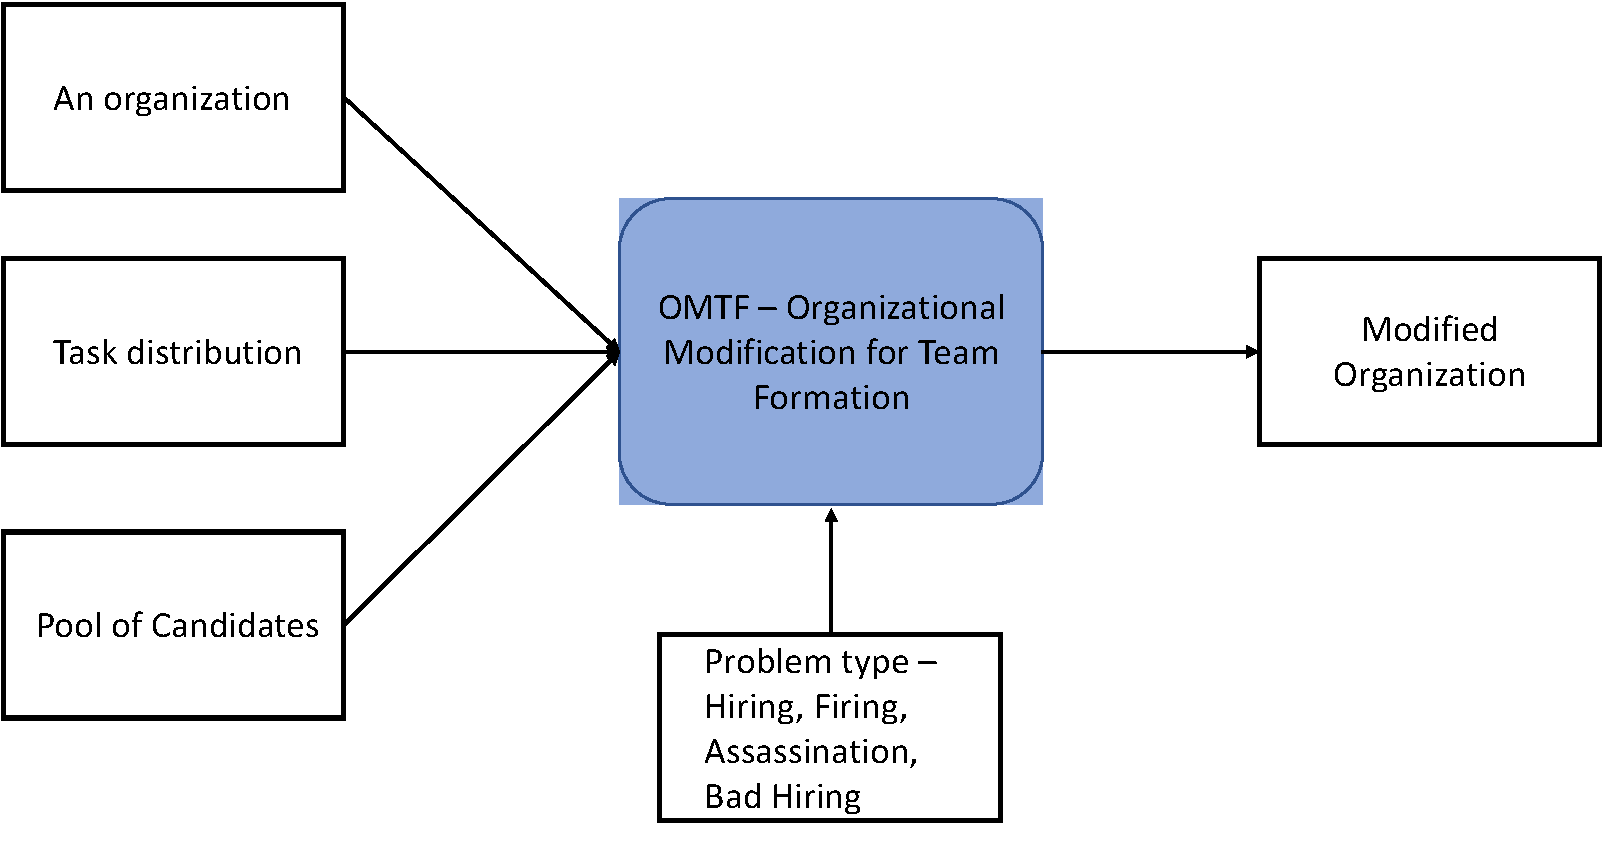
\includegraphics[width=1.0\textwidth]{figs/illustration.pdf}
\caption{Framework of our proposed system}
\label{fig:hpo}
\end{small}
\end{figure} 

Unfortunately optimizing all the four objectives are NP-hard. Hence we resort to approximation strategies. Recently in \cite{bai2016algorithms} authors have produced a simple greedy approximation that preserves a $1 - \frac{1}{e}$ - approximation while optimizing an objective that is the ratio of submodular functions. Now under properly chosen utility and cost functions, the objective of team formation problem turns out to be a ratio of submodular functions. Thus we base our algorithm on that approach. However organization creates an added layer of complexity. Our aim is to optimize the decision we make for the organization, which in turn depends on the optimum allocation of the resources to the tasks. The second optimization can be approximated using the proposed algorithm of \cite{bai2016algorithms}. However the presence of the outer optimization breaks the approximation guarantee. To circumvent this issue, we use greedy heuristics, that leverage the combinatorial structure of the problems. This algorithm does not have a provable bound, but we show that in real-world datasets it performs quite well.

Thus, to summarize, our contributions are the following:

\begin{enumerate}
\item We formulate the novel \textit{hiring, firing, assassination and bad hiring problems}, in context of an organization, which draws inspirations from the team formation literature.

\item We show that the problems are NP-hard. However, under certain communication and coverage functions, we can get, efficient approximation algorithms can be designed for the problems.

\item By leveraging the work of \cite{bai2016algorithms}, we develop a greedy heuristic to solve the problems. We show that because of the presence of an additional optimization requirement, the $(1 - \frac{1}{e})$ approximation guarantee of \cite{bai2016algorithms} does not carry forward. However by exploiting the combinatorial nature of our problem we develop an efficient greedy heuristic.

\item We experimentally validate our approach on real-world dataset. 

\end{enumerate}